\documentclass{article}
\usepackage[margin=0.5in]{geometry}
\usepackage{pgfplots}

	\pgfplotsset{
    discard if not/.style 2 args={
        x filter/.code={
            \edef\tempa{\thisrow{#1}}
            \edef\tempb{#2}
            \ifx\tempa\tempb
            \else
                \def\pgfmathresult{inf}
            \fi
        }
    }
}

\begin{document}

% \pgfplotsset{width=3in}
% \pgfplotsset{height=7.5in}
% \begin{tikzpicture}
% \begin{axis}[
% 			title=Copper,
% 			ylabel=Energy $(Ry)$,
% 			% ymin=-0.2,
% 			% ymax = 1.,
% 			% xtick={0,50,100,125,150,175,200,225,250},
% 			% xticklabels={$\Gamma$,$\Delta$,$X$,$Z$,$W$,$Q$, $L$,$\Lambda$, $\Gamma$},
% 		]
% % \addplot [thick, black, discard if not={P}{A}] table [x=X, y=Y] {moosles.txt};
% % \addplot [thick, red, discard if not={P}{B}] table [x=X, y=Y] {moosles.txt};
% % \addplot [thick, blue, discard if not={P}{C}] table [x=X, y=Y] {moosles.txt};
% % \addplot [thick, purple, discard if not={P}{D}] table [x=X, y=Y] {moosles.txt};
% % \addplot [thick, orange, discard if not={P}{E}] table [x=X, y=Y] {moosles.txt};
% % \addplot [thick, gray, discard if not={P}{F}] table [x=X, y=Y] {moosles.txt};
% % \addplot [thick, blue, discard if not={P}{G}] table [x=X, y=Y] {moosles.txt};
% % \addplot [thick, red, discard if not={P}{H}] table [x=X, y=Y] {moosles.txt};
% % \addplot [thick, purple, discard if not={P}{I}] table [x=X, y=Y] {moosles.txt};
% \addplot [thick, black] table [x=x1, y=x2] {bands.CoCu100};
% \addplot [thick, red] table [x=x1, y=x3] {bands.CoCu100};
% \addplot [thick, blue] table [x=x1, y=x4] {bands.CoCu100};
% \addplot [thick, purple] table [x=x1, y=x5] {bands.CoCu100};
% \addplot [thick, orange] table [x=x1, y=x6] {bands.CoCu100};
% \addplot [thick, gray] table [x=x1, y=x7] {bands.CoCu100};
% \addplot [thick, blue] table [x=x1, y=x8] {bands.CoCu100};
% \addplot [thick, red] table [x=x1, y=x9] {bands.CoCu100};
% \addplot [thick, purple] table [x=x1, y=x10] {bands.CoCu100};
% % \addplot [thick, black, discard if not={P}{J}] table [x=X, y=Y] {moosles.txt};
% % \addplot [thick, red, discard if not={P}{K}] table [x=X, y=Y] {moosles.txt};
% % \addplot [thick, blue, discard if not={P}{L}] table [x=X, y=Y] {moosles.txt};
% % \addplot [thick, purple, discard if not={P}{M}] table [x=X, y=Y] {moosles.txt};
% % \addplot [thick, orange, discard if not={P}{N}] table [x=X, y=Y] {moosles.txt};
% % \addplot [thick, gray, discard if not={P}{O}] table [x=X, y=Y] {moosles.txt};
% % \addplot [thick, blue, discard if not={P}{P}] table [x=X, y=Y] {moosles.txt};
% % \addplot [thick, red, discard if not={P}{Q}] table [x=X, y=Y] {moosles.txt};
% % \addplot [thick, purple, discard if not={P}{R}] table [x=X, y=Y] {moosles.txt};
% \end{axis}
% \end{tikzpicture}

% \begin{tikzpicture}
% \begin{axis}
% [
% 			title=Copper,
% 			ylabel=Energy $(Ry)$,
% 			% ymin=-0.2,
% 			% ymax = 1.,
% 			xtick={0,50,100,125,150,175,200,225,250},
% 			xticklabels={$\Gamma$,$\Delta$,$X$,$Z$,$W$,$Q$, $L$,$\Lambda$, $\Gamma$},
% 			% xmax = 100,
% 		]
% \addplot [thick, black, discard if not={P}{A}] table [x=X, y=Y] {test.txt};
% \addplot [thick, red, discard if not={P}{B}] table [x=X, y=Y] {test.txt};
% \addplot [thick, blue, discard if not={P}{C}] table [x=X, y=Y] {test.txt};
% \addplot [thick, purple, discard if not={P}{D}] table [x=X, y=Y] {test.txt};
% \addplot [thick, orange, discard if not={P}{E}] table [x=X, y=Y] {test.txt};
% \addplot [thick, gray, discard if not={P}{F}] table [x=X, y=Y] {test.txt};
% \addplot [thick, blue, discard if not={P}{G}] table [x=X, y=Y] {test.txt};
% \addplot [thick, red, discard if not={P}{H}] table [x=X, y=Y] {test.txt};
% \addplot [thick, purple, discard if not={P}{I}] table [x=X, y=Y] {test.txt};
% 	\end{axis}
% \end{tikzpicture}


% \pgfplotsset{width=5in}
% \pgfplotsset{height=5in}
% \begin{tikzpicture}
% 	\begin{axis}[
% 			title = Exchange Coupling in Co/Cu/Co(100),
% 			ylabel style = {yshift=1cm},
% 			ylabel = J(n) \quad $(Ry)$,
% 			xlabel = Spacer thickness \quad (n),
% 			scaled y ticks = false,
% 			xmin = 3,
% 			xmax = 35,
% 		]
% 		\addplot [thick, green] table [col sep=comma] {Eff.txt};\addlegendentry{Mobius transformation method for continuous n}
% 		\addplot [only marks, fill=red] table [col sep=comma] {Ef.txt};\addlegendentry{Adlayer method for integer n}
% 	\end{axis}
% \end{tikzpicture}

% \pgfplotsset{width=6in}
% \pgfplotsset{height=2in}
% \begin{tikzpicture}
% 	\begin{axis}[
% 			title = Total DOS in FCC Cu direct 3D,
% 			ylabel = DOS,
% 			xlabel = Energy \qquad $(Ry)$,
% 			scaled y ticks = false,
% 			ymin =0,
% 			ymax=100,
% 			xmin = -0.2,
% 			xmax=1.1,
% 			scaled x ticks = false,
% 			x tick label style={
% 			/pgf/number format/fixed,
% 		/pgf/number format/precision = 2},
% 		]
% 		     \addplot +[black,mark=none, dashed] coordinates {(0.5805, 0) (0.5805, 100)};
% 		     % \addplot [thick] table {tdosrem2.txt};
% 		     \addplot [thick] table {mnm.txt};
% 		     \addplot [thick] table {mmm.txt};
% 	\end{axis}
% \end{tikzpicture}

% \pgfplotsset{width=6in}
% \pgfplotsset{height=6in}
% \begin{tikzpicture}
% 	\begin{axis}[
% 			% title = Total DOS in FCC Cu 2D diagonalised in-plane,
% 			title = Partial DOS, 
% 			ylabel = DOS,
% 			xlabel = Energy \qquad $(Ry)$,
% 			scaled y ticks = false,
% 			% ymin =0,
% 			% ymax=100,
% 			% xmin = 0,
% 			% xmax=1,
% 			scaled x ticks = false,
% 			x tick label style={
% 			/pgf/number format/fixed,
% 		/pgf/number format/precision = 2},
% 		]
% 		     % \addplot +[black,mark=none, dashed] coordinates {(0.5805, 0) (0.5805, 100)};
% 		     \addplot [thick] table {X.txt};
% 		     % \addplot [thick] table {rem.txt};
% 	\end{axis}
% \end{tikzpicture}

% \begin{figure}[h]
% 	\begin{center}
% 		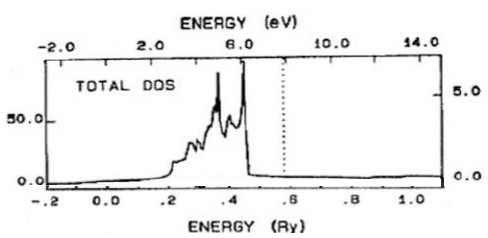
\includegraphics{Cu.jpg}
% 	\end{center}
% \end{figure}

% \pgfplotsset{width=5in}
% \pgfplotsset{height=5in}
% \begin{tikzpicture}
% 	\begin{axis}[
% 			title = Exchange Coupling in FCC CoCuCo(100),
% 			ylabel = J \qquad $(mRy)$,
% 			ylabel style = {yshift=1cm},
% 			xlabel = Chemical potential in the LH lead \qquad $(Ry)$,
% 			scaled y ticks = false,
% 			scaled x ticks = false,
% 			% yticklabels = {0.05, 0.04, 0.03, 0.02, 0.01, 0, -0.01, -0.02, -0.03},
% 		y filter/.code={\pgfmathparse{#1*1000}\pgfmathresult},
% 			% y dir = reverse,
% 			y tick label style={
% 			/pgf/number format/fixed,
% 		/pgf/number format/precision = 3},
% 			x tick label style={
% 			/pgf/number format/fixed,
% 		/pgf/number format/precision = 2},
% 			% ymin =0,
% 			% ymax=100,
% 			xmin = -0.04,
% 			xmax=0.06,
% 			legend style = {at={(0.03,0.9)},anchor=west},
% 		]
% 		\addplot [thick] table {phase3_diamond.txt};\addlegendentry{Co/Cu(6)/Co}
% 		     \addplot [red,thick] table {phase5_diamond.txt};\addlegendentry{Co/Cu(10)/Co}
% 		     \addplot [blue,thick] table {phase7_diamond.txt};\addlegendentry{Co/Cu(14)/Co}
% 		% \addplot [thick] table {newEC_6.txt};\addlegendentry{Co/Cu(6)/Co}
% 		     % \addplot [red,thick] table {newEC_10.txt};\addlegendentry{Co/Cu(10)/Co}
% 		     % \addplot [blue,thick] table {newEC_14.txt};\addlegendentry{Co/Cu(14)/Co}
% 	\end{axis}
% \end{tikzpicture}

% \pgfplotsset{width=5in}
% \pgfplotsset{height=5in}
% \begin{tikzpicture}
% 	\begin{axis}[
% 			% title = Partial Exchange Coupling in FCC CoCuCo(100) with $k_x = 0, k_z = 0$ and the first Matsubara term only,
% 			ylabel = J \qquad $(mRy)$,
% 			ylabel style = {yshift=1cm},
% 			xlabel = Spacer layer thickness \qquad $(n)$,
% 			scaled y ticks = false,
% 			% scaled x ticks = false,
% 			% yticklabels = {0.05, 0.04, 0.03, 0.02, 0.01, 0, -0.01, -0.02, -0.03},
% 		y filter/.code={\pgfmathparse{#1*1000}\pgfmathresult},
% 			% y dir = reverse,
% 			y tick label style={
% 			/pgf/number format/fixed,
% 		/pgf/number format/precision = 3},
% 			% x tick label style={
% 			% /pgf/number format/fixed,
% 		% /pgf/number format/precision = 2},
% 			ymin =-5,
% 			% ymax=100,
% 			% xmin = -0.04,
% 			xmax=30,
% 			% legend style = {at={(0.03,0.9)},anchor=west},
% 		]
% 		\addplot [thick] table {res};\addlegendentry{Andrey's results}
% 		     \addplot [red,thick] table {tes.txt};\addlegendentry{Alex's results}
% 		     % \addplot [blue,thick] table {phase7_diamond.txt};\addlegendentry{Co/Cu(14)/Co}
% 		% \addplot [thick] table {newEC_6.txt};\addlegendentry{Co/Cu(6)/Co}
% 		     % \addplot [red,thick] table {newEC_10.txt};\addlegendentry{Co/Cu(10)/Co}
% 		     % \addplot [blue,thick] table {newEC_14.txt};\addlegendentry{Co/Cu(14)/Co}
% 	\end{axis}
% \end{tikzpicture}

% \pgfplotsset{width=5in}
% \pgfplotsset{height=5in}
% \begin{tikzpicture}
% 	\begin{axis}[
% 			% title = Partial Exchange Coupling in FCC CoCuCo(100) with $k_x = 0, k_z = 0$ and the first Matsubara term only,
% 			ylabel = J \qquad $(mRy)$,
% 			ylabel style = {yshift=1cm},
% 			xlabel = Spacer layer thickness \qquad $(n)$,
% 			scaled y ticks = false,
% 			% scaled x ticks = false,
% 			% yticklabels = {0.05, 0.04, 0.03, 0.02, 0.01, 0, -0.01, -0.02, -0.03},
% 		y filter/.code={\pgfmathparse{#1*1000}\pgfmathresult},
% 			% y dir = reverse,
% 			y tick label style={
% 			/pgf/number format/fixed,
% 		/pgf/number format/precision = 3},
% 			% x tick label style={
% 			% /pgf/number format/fixed,
% 		% /pgf/number format/precision = 2},
% 			ymin =-0.5,
% 			ymax=0.5,
% 			xmin = 4,
% 			xmax=30,
% 			% legend style = {at={(0.03,0.9)},anchor=west},
% 		]
% 		\addplot [thick] table {res};\addlegendentry{Andrey's results}
% 		     \addplot [red,thick] table {tes.txt};\addlegendentry{Alex's results}
% 		     % \addplot [blue,thick] table {phase7_diamond.txt};\addlegendentry{Co/Cu(14)/Co}
% 		% \addplot [thick] table {newEC_6.txt};\addlegendentry{Co/Cu(6)/Co}
% 		     % \addplot [red,thick] table {newEC_10.txt};\addlegendentry{Co/Cu(10)/Co}
% 		     % \addplot [blue,thick] table {newEC_14.txt};\addlegendentry{Co/Cu(14)/Co}
% 	\end{axis}
% \end{tikzpicture}

\pgfplotsset{width=6in}
\pgfplotsset{height=6in}
\begin{tikzpicture} 
	\begin{axis}[
			% title=Adaptive Cunningham Points based quadrature routine developed by the author,
			ylabel=$k_z$,
			ylabel style={rotate=-90},
			xlabel=$k_x$,
			% xtick={0,1.5708,3.14159},
			% xticklabels={$0$,$\frac{\pi}{2}$,$\pi$},
			% ytick={0,1.5708,3.14159},
			% yticklabels={$0$,$\frac{\pi}{2}$,$\pi$},
			% ymin=-0.2,
			% ymax=3.34,
			% xmin=-0.2,
			% xmax=3.34,
		]
		\addplot[only marks, mark size=0.7pt,violet] table  {best_to_keep_for_adaptive_demo.txt};
	\end{axis}
\end{tikzpicture}




\end{document}
